\documentclass[a4paper, 12pt]{article}

\usepackage{wrapfig}
\usepackage{graphicx}
\usepackage{mathtext}
\usepackage{amsmath}
\usepackage{siunitx} % Required for alignment
\usepackage{multirow}
\usepackage{gensymb}
\usepackage{rotating}
\sisetup{
  round-mode          = places, % Rounds numbers
  round-precision     = 2, % to 2 places
}

\usepackage[T1,T2A]{fontenc}

\usepackage[russian]{babel}

\graphicspath{{pictures/}}


\title{\begin{center}Лабораторная работа №1.2.5\end{center}
Иследование прецессии уравновешенного гироскопа}
\author{Гёлецян А.Г.}
\date{\today}

\begin{document}
    \pagenumbering{gobble}
    \maketitle
    \newpage
    \pagenumbering{arabic}

    \section{Ход работы}
    \paragraph{}
    Сначала установим параметры системы.
    \begin{align*}
     l&=(112\pm1)мм\\
     g&=(9.8155\pm0.0005)мс^{-2}\\
     \Delta m &= 1г\\
     \varepsilon_T &= 1\%
    \end{align*}

    \paragraph{}
    Приведем данные, полученные при измерениях.

    \begin{table}[h!]
        \begin{center}
        \begin{tabular}{|l|r|r|r|r|r|r|}
        \hline
        $№$ & $m, г$ &   $N$ & $t, с$ & $\alpha, \degree$ & $\Delta \alpha, \degree$ & $T, с$\\\hline
        1  &  342 &  11 &  335 &   9 &      1 &  30.5 \\
        2  &  342 &  12 &  365 &   9 &      1 &  30.4 \\
        3  &  274 &  11 &  419 &  10 &      1 &  38.1 \\
        4  &  274 &  11 &  414 &  10 &      1 &  37.6 \\
        5  &  220 &   8 &  378 &  10 &      1 &  47.2 \\
        6  &  220 &  10 &  468 &  10 &      1 &  46.8 \\
        7  &  179 &   7 &  406 &  10 &      1 &  58.0 \\
        8  &  179 &   7 &  408 &  10 &      1 &  58.3 \\
        9  &  142 &   5 &  368 &  10 &      1 &  73.6 \\
        10 &  142 &   6 &  441 &  10 &      1 &  73.5 \\
        \hline
        \end{tabular}
         \caption{Измерения периода прецессии при различных массах груза}
        \end{center}

    \end{table}

    \paragraph{}
    Отсюда обработав данные получаем следующие значения


    \begin{table}[h!]
        \begin{center}
        \begin{tabular}{|l|r|r|r|r|r|r|r|}
        \hline
        $№$ & $m, г$ &   $T, с$ & $\Delta T, с$ & $\Omega, с^{-1}$ & $\Delta\Omega, с^{-1}$ & $M, Нм$ & $\Delta M, Нм$\\\hline
        1 &  142 &  73.6 &    0.7 &  0.085 &  0.001 &  0.169 &  0.002 \\
        2 &  179 &  58.1 &    0.6 &  0.108 &  0.001 &  0.213 &  0.002 \\
        3 &  220 &  47.0 &    0.5 &  0.134 &  0.001 &  0.261 &  0.002 \\
        4 &  274 &  37.9 &    0.4 &  0.166 &  0.002 &  0.325 &  0.003 \\
        5 &  342 &  30.4 &    0.3 &  0.207 &  0.002 &  0.406 &  0.004 \\
        \hline
        \end{tabular}
         \caption{Обработанные данные}
        \end{center}

    \end{table}
    \paragraph{}
    В таблице выше были использованы следующие формулы

    \begin{align*}
     \Omega &= \frac{2\pi}{T}\\
     \Delta \Omega &= \Omega \frac{\Delta T}{T}\\
     M &= mgl\\
     \Delta M &= M \sqrt{\left(\frac{\Delta m}{m}\right)^2 +
                        \left(\frac{\Delta g}{g}\right)^2 +
                        \left(\frac{\Delta l}{l}\right)^2}
    \end{align*}

    \paragraph{}
    Теоретически есть зависимость между $\Omega$ и $M$. Выглядит оно по следующему
    \[\Omega = \frac{M}{L}\]
    где
    \[L = I_{ротор}\omega_{ротор}\]
    \paragraph{}
    Построив график $\Omega(M)$ получаем значение $1/L$.
    \[\frac{1}{L}=(0.509 \pm 0.005)(Нмс)^{-1}\].
    \subsection{Измерение частоты вращения ротора}

    \paragraph{}
    Теперь измерим момент инерции ротора для дальнейших обработок. Измерять будем крутильным маятником, предварительно "отколибровав" его цилиндром с известным моментом инерции.

    Для цилиндра имеем
    \begin{align*}
     m_{ц} &= (1617.8 \pm 0.1)г\\
     d_{ц} &= (7.80 \pm 0.01)см\\
     I_{ц} &= \frac{md^2}{8} = (1.230 \pm 0.003) 10^{-3} кгм^2\\
    \end{align*}
    Измерив периоды колебании цилиндра и ротора посчитаем момент инерции ротора
    \begin{align*}
     T_{ц} &= (4.07 \pm 0.01)с\\
     T_{р} &= (3.22 \pm 0.01)с\\
     I_{р} &= I_{ц} \frac{{T_р}^2}{{T_ц}^2} = (0.771 \pm 0.006)10^{-3} кгм^2
    \end{align*}
    \paragraph{}
    Если обозначим $x=1/L$ то частота вращения ротора поучается
    \[\nu = \frac{1}{2\pi I_р x} = (405 \pm 5)Гц\]

    \paragraph{}
    При измерении этой частоты осцилографом с помощью фигур лиссажу получаем значение
    \[\nu_{осц}=(389 \pm 1)Гц\]

    \subsection{Измерение момента трения}
    \paragraph{}
    Во время эксперимерта ось гироскопа опускалось в первую очередь из за трения в вертикальной оси. Для оценивания момента сил трения можно воспользоватся данными про угол наклона $\alpha$ за время эксперимента $t$. Формула момента трения приобретает следующий вид.
    \[M_{тр} \approx \frac{L\alpha}{t}\]
    Для наших данных получаем следующие значения.


    \begin{table}[h!]
        \begin{center}
        \begin{tabular}{|l|r|r|r|r|r|r|r|r|r|r|}
        \hline
        $M_{тр}, 10^{-4}Нм$ &  9.0 &  8.0 &  8.0 &  8.0 &  9.0 &  7.0 &  8.0 &  8.0 &  9.0 &  8.0 \\\hline
        $\Delta M_{тр}, 10^{-4}Нм$ &  1.0 &  1.0 &  1.0 &  1.0 &  1.0 &  1.0 &  1.0 &  1.0 &  1.0 &  1.0 \\
        \hline
        \end{tabular}
         \caption{Моменты сил трения}
        \end{center}

    \end{table}
    \paragraph{}
    Усредняя получаем
    \[M_{тр}=(8.2 \pm 1.2) 10^{-4}Нм\]
    \section{Заключение}
    Как видим частоты вращения близки, но в пределах погрешности они не совпадают. В чем причина расхождения? Пытатся объяснить тем, что мы не учитываем косинус угла при подсчете момента, или тем что угловая скорость прецессии в этом виновата не получится, слишком мелкие поправки. По моему мнению проблема состоит в измерении момента инерции ротора, так как при неуравновешенных колебаниях момент инерции искажается.


    \newpage
    \begin{sidewaysfigure}
        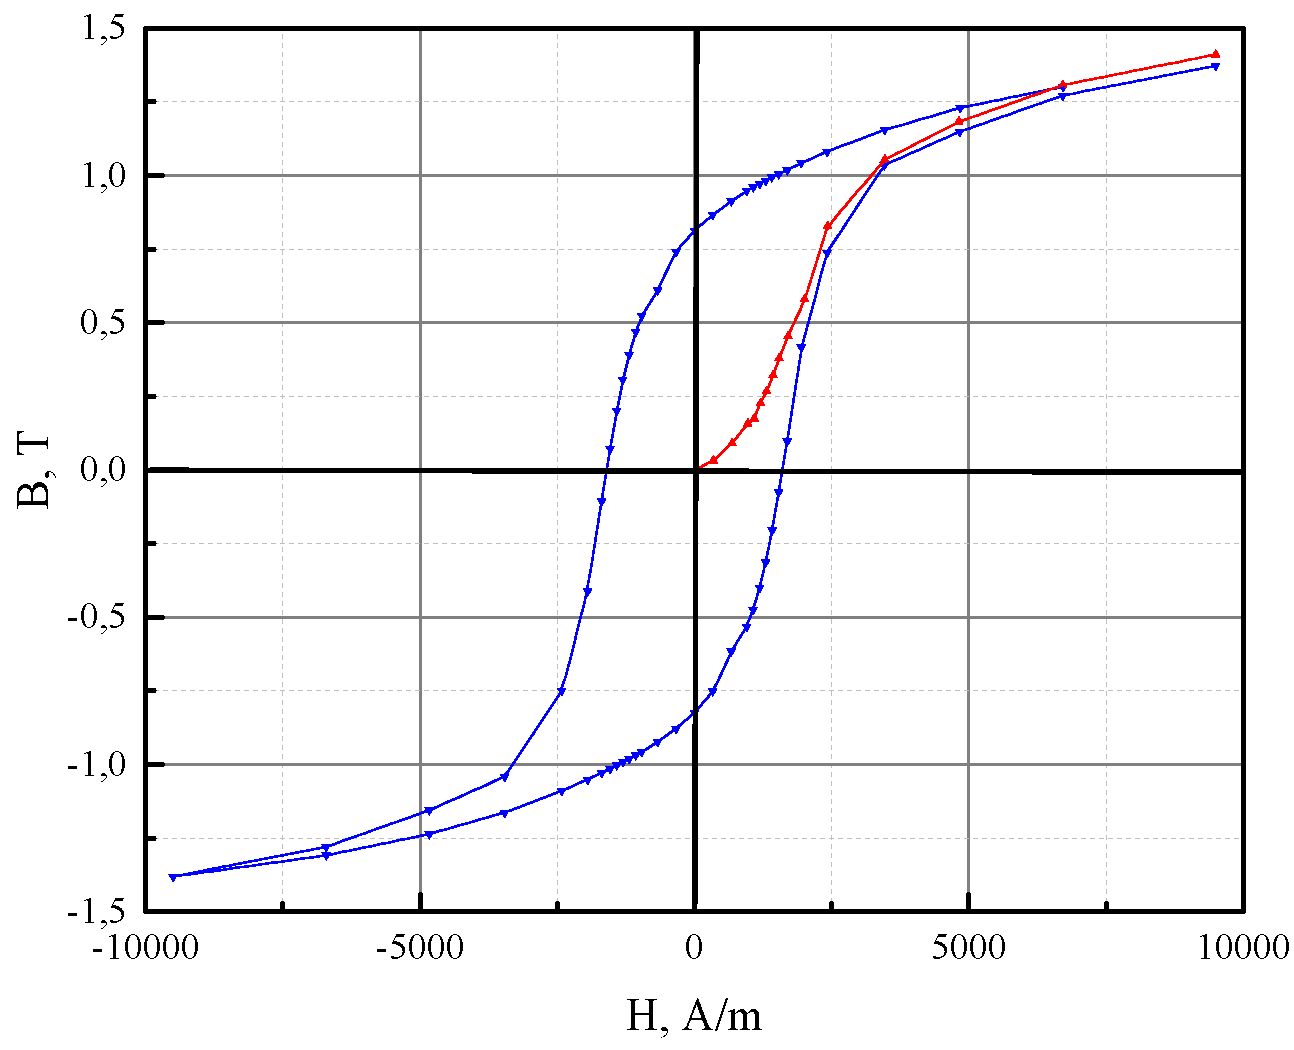
\includegraphics[width=1.20\textwidth]{plot.png}
        \caption{График $\Omega(M)$}
    \end{sidewaysfigure}
\end{document}

